\chapter{Opis projektnog zadatka}
		


{Ovaj se projekt bavi razvojem programske podrške za web aplikaciju "TectonicHR". 
	Cilj aplikacije "TectonicHR" olakšano je prikupljanje podataka o intenzitetu potresa te olakšani vizualni pristup informacijama. 
	Aplikacija je namijenjena znanstvenoj zajednici, ali i općoj populaciji.
	
	 
	Znanstvenoj zajednici, seizmolozima, bit će olakšan pristup informacijama i njihovo prikupljanje.  
	Opća populacija, građani, imat će mogućnost unosa novog potresa kojega su osjetili te pregled već zabilježenih potresa.  
	
	
	Prilikom otvaranja aplikacije građanima se nude tri opcije te se pokazuje preliminarna karta Hrvatske na kojoj su označeni aktualni i arhivirani potresi. Boje oznaka potresa različite su za ove dvije kategorije potresa.
	Prva opcija, „Aktualni potresi“, omogućava pregled aktualnih potresa te ispunjavanje upitnika za njih. 
	Druga opcija, „Arhivirani potresi“, otvara stranicu koja prikazuje pregled preliminarne karte inteziteta potresa koja sadži interaktivnu kartu Hrvatske te popis arhiviranih potresa. 
	Na karti je zvjezdicom označen epicentar te kružićem određene boje označen je intenzitet potresa. (Hladnije plave nijanse označavaju slabiji intezitet, a tamnije crvene jači intezitet). 
	Ispod karte nalazi se tablica s podacima o zadnjem i starijim potresima. Pri pregledu arhiviranih i aktualnih potresa moguće je filtrirati potrese prema mjestu, vremenu ili intezitetu. 
	Ako se zadnji potres ne poklapa s opažanjima građana, preko treće opcije „Novi potres?" građanin može dodati novi potres koji je osjetio. 
	Kada građanin odluči dodati novi potres, obavezan je popuniti i predati upitnik. 
	Upitnik se sastoji od pitanja iz kojih znanstvenici mogu dobiti vrijedne informacije o tome kakvi su bili učinci potresa. 
	Pitanja se odnose na to koliko se potres osjetio, koliku je štetu napravio na malim predmetima, kućama, zgradama i zemlji te kako su ljudi reagirali. 
	Odgovori na ta pitanja pomažu pri računanju intenziteta potresa. 
	Na početnoj stranici u gornjem desnom kutu nalazi se gumb za prijavu u sustav. Tu funkcionalnost koriste seizmolozi koji žele preuzeti podatke o potresu i odgovore građana.  Pri prijavi upisuju svoje ime, prezime, email, korisničko ime i lozinku. 
	Znanstvenike u sustav mora registrirati administrator kako neovlaštena osoba ne bi mogla pristupiti svim podacima. Nakon što se seizmolog registrira u sustav, administrator će ga e-mailom obavijestiti je li registracija potvrđena ili odbijena. 
	Pregled svih registriranih seizmologa omogućen je samo administratoru.
	Administrator se također mora prijaviti pri dolasku na stranicu kako bi imao sve ovlasti. \\
	
	}
	
	Program treba sam računati intenzitet potresa pomoću prethodno preuzetih upitnika. Upitnik treba automatski izračunati i proslijediti intenzitet potresa prema odgovorenim pitanjima. 
	Vrijednost intenziteta na pojedinoj lokaciji odgovara srednjoj vrijednosti intenziteta svih upitnika ispunjenih za potres na istoj lokaciji. Mjesto epicentra aproksimira se koristeći lokacije jednakog intenziteta, a intenzitet potresa se u epicentru (predstavljen bojom) određuje koristeći \textit{Koevesligethyjevu jednadžbu}:
\begin{equation}
  I_{0} = I_{max} + 3\log\frac{r}{h} + 3\mu\alpha(r-h)
\end{equation}

\begin{itemize}                                                             
    \item $I_{max}$ - procijenjeni intenzitet potresa na udaljenosti r od hipocentra
    \item h = 10 km 
    \item $\mu=0.4343$
    \item $\alpha=0.005 km^{-1}$
    
\end{itemize} 


\section{Vrste korisnika}
Postoje tri vrste korisnika, a to su:
\begin{packed_item}
	\item anonimni korisnik (građanin)
	\item znanstvenik (seizmolog)
	\item administrator
\end{packed_item}

\underbar{Neregistriranom (anonimnom) korisniku} otvaranjem aplikacije prikazuje se izbornik u kojem može odabrati želi li pregledati aktualne potrese („Aktualni potresi“), pregledati arhivirane potrese („Arhivirani potresi“) ili ispuniti upitnik ako je osjetio novi potres („Novi potres?“). Klikom na „Aktualni potresi“ prikazuju mu se karta i popis potresa koje administrator još nije arhivirao. Anonimni korisnik može pretraživati te potrese i odabrati jedan potresa te za njega ispuniti upitnik. Na početnoj stranici, klikom na „Arhivirani potresi“ pokaže mu se karta i ispod nje popis potresa koje je administrator arhivirao. Prelaženjem kursorom preko oznake kojom je označen taj potres, prikazuju mu se osnovne informacije o potresu (datum, vrijeme, lokacija i intenzitet potresa).

\underbar{Seizmolog (znanstvenik)} se prijavljuje e-mailom i lozinkom. Seizmolog klikom na ikonu u kutu početnog zaslona odlazi na svoj profil gdje mu se omogućuje prikaz i promjena osobnih podataka (korisničko ime, ime, prezime, e-mail, lozinka). Ima sve mogućnosti kao i anonimni korisnik (ispunjavanje upitnika za novi potres, pregled karte i drugih podataka o aktualnim i arhiviranim potresima) uz još dodatnu ovlast preuzimanja podataka o potresima u .csv formatu.

\underbar{Administrator} ima najveće ovlasti. Početna stranica izgleda mu isto kao i seizmologu, ali mu se na stranici profila ispod njegovih podataka nalaze i dva gumba, „Novi upitnici“ i „Nove prijave“. Klikom na „Novi upitnici“ pregledava ispunjene upitnike koje još nije svrstao u nijedan potres. Upitnike može pridijeliti nekom već imenovanom potresu ili može stvoriti, imenovati i potvrditi novi potres te ih pridijeliti tom novostvorenom potresu. Klikom na „Nove prijave“ prikazuje mu se popis osoba koje žele biti registrirane kao znanstvenici. Odabirom jedne ili više prijava može ih registrirati. S početne stranice može pristupiti stranici aktualnih potresa. Na toj stranici može odabrati jedan ili više potres te ih arhivirati. Na stranici arhiviranih potresa može pregledavati i izmjenjivati podatke o starim potresima te također, kao i seizmolog, preuzeti podatke .csv formatu.

Sustav treba podržavati rad više korisnika u stvarnom vremenu.\\



\section{Usporedba s već postojećim rješenjima}

{Od sličnih aplikacija koje već postoje, najpoznatija je EMSC. Aplikaciju je razvila organizacija European Mediterranean Seismological Centre. 
Početna stranica sastoji se od karte Europe i Mediterana. Na karti možete birati želite li pregledati potrese u zadnjih sat  vremena, 24 sata, 48 sati, tjedan dana ili dva tjedna. Osim karte Europe i Mediterana, postoji mogućnost otvaranja karte cijelog svijeta. 
Ispod karte nalazi se tablica s informacijama o potresima koji su označeni na karti. Osim toga, stranica nudi funkcionalnosti ispunjavanja upitnika o doživljaju potresa i dodavanje slika koje prikazuju posljedice potresa. Postoji posebni odjeljak za seizmologe, kao i odjeljci namijenjeni projektima organizacije i publikaciji. Problem stranice je što je prilično neintuitivna za korištenje i zastarjelog dizajna. Nudi mnogo mogućnosti u raznim izbornicima te to stvara mogućnost nesnalaženja. Većinu građana koji posjećuju tu stranicu radi prijave potresa ili traženja informacija o potresu kojega su možda osjetili, zasigurno neće zanimati projekti EMSC-a ili publikacija.}

\begin{figure}[H]
			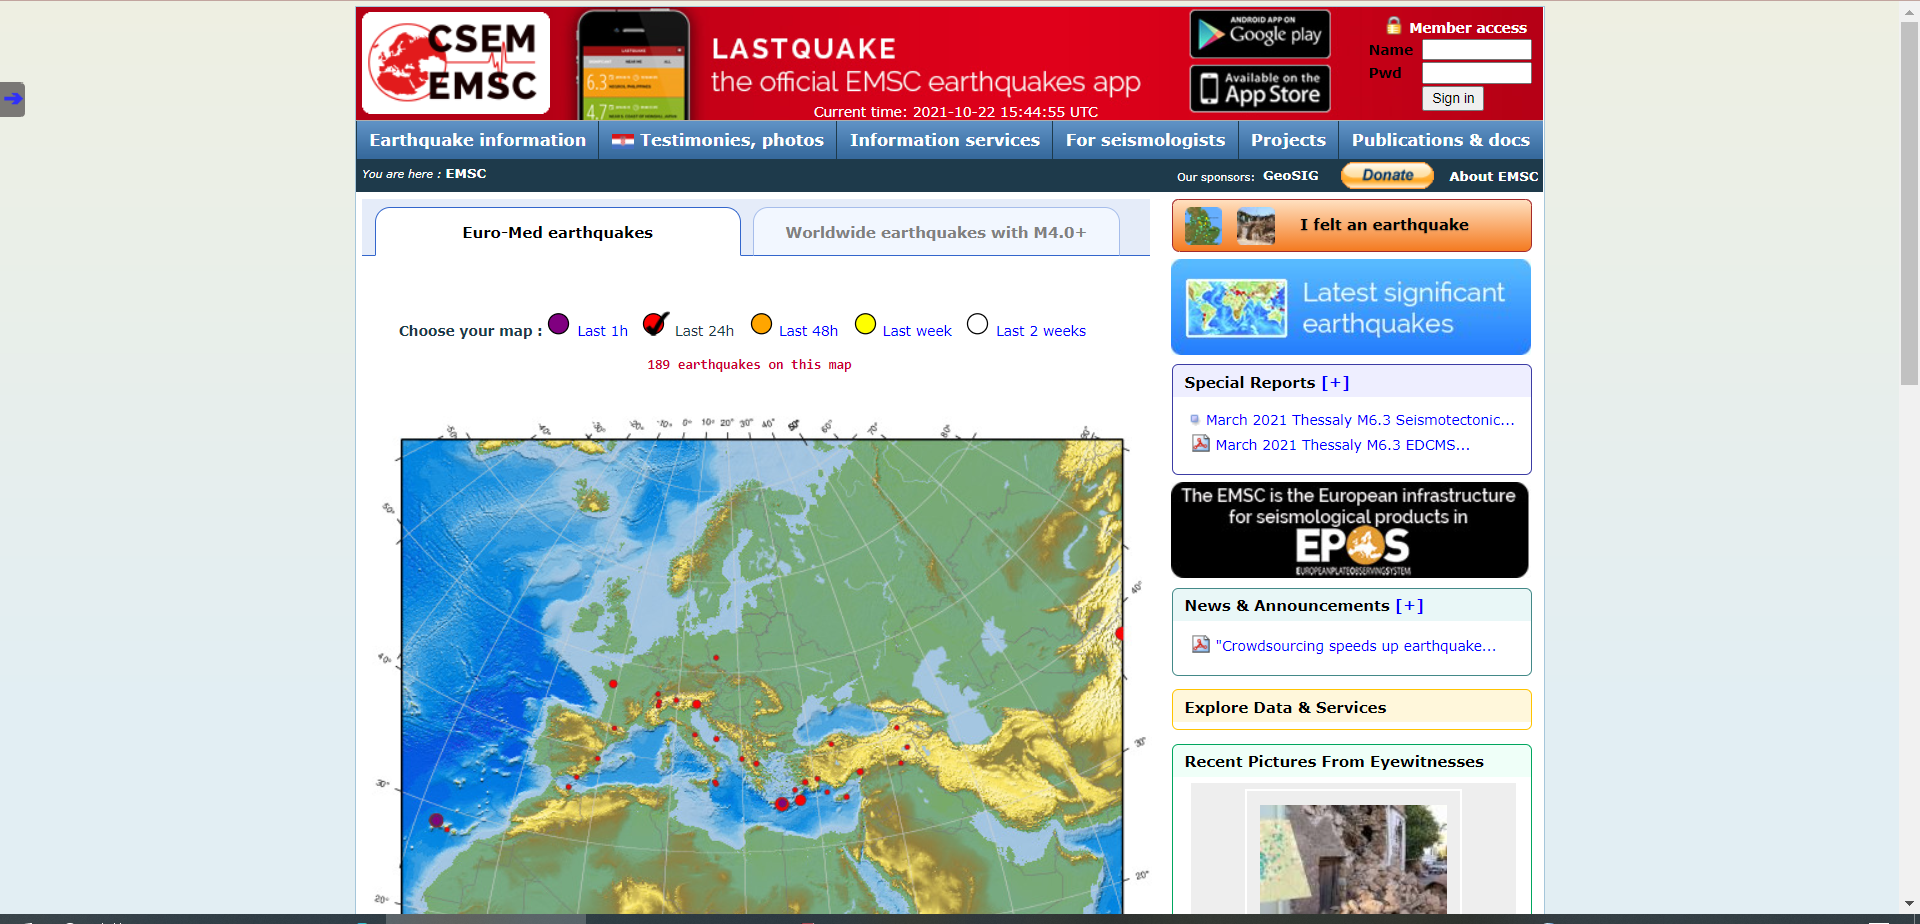
\includegraphics[width=\textwidth]{slike/emsc1.PNG} %veličina u odnosu na širinu linije
			\caption{Slika 2.2: početna stranica EMSC-a}
			\label{fig:promjene2} %label mora biti drugaciji za svaku sliku
		\end{figure}

{Prednost aplikacije „TectonicHR“ bila bi preglednost i mogućnost lakšeg snalaženja na karti. 
Mogućnost prijave seizmologa na stranicu omogućilo bi bolju prilagodbu stranice. Građanima pri korištenju ne bi smetali izbornici s mogućnostima koje oni ne bi koristili, već bi im se pregledno prikazivale funkcionalnosti dodavanja potresa i pregleda aktualnih i starijih potresa. }

{Interes za korištenjem aplikacije imat će i građani i znanstvena zajednica. Potresi uvelike utječu na psihičko stanje ljudi. 
Kada dođe do potresa, većina želi znati gdje je epicentar, koliko je magnitude potres bio, kakvu je štetu prouzročilo u ostalim dijelovima pogođenog područja… 
Tako da bi ova jednostavna aplikacija ljudima pružila, za početak, osnovne informacije o doživljenom potresu te odgovor na neka od pitanja koja im se nameću nakon doživljenog potresa. 
Osim toga, korist od aplikacije imaju i znanstvenici koji putem opažanja građana mogu doći do vrlo vrijednih informacija. }\\		
		
\eject
		
	